\documentclass[11pt, twoside, a4paper]{report}

\usepackage{float}

\usepackage{verbatim}
\usepackage{tikz}
\usetikzlibrary{arrows,shapes}
\tikzstyle{vertex} = [circle, fill=black!25, minimum size=100pt, inner sep=0pt]
\tikzstyle{edge} = [draw, thick, line width=1.5pt, inner sep=5pt, outer sep=5pt]

\begin{document}

\title{\textbf{Perceiving and memorising packaged goods} \\ (in a supermarket environment) \\ \vspace{7.5mm} \textsc{Diploma Thesis}}
\author{Carsten K\"onemann \\ \texttt{cargath@gmail.com}}
\date{08.10.2013}

\maketitle

\chapter{Abstract}

\tableofcontents

\chapter{Introduction}

\section{Review}
Current solutions can be divided into two groups: Those which search for a specific object as needed, and those which utilize a set of predetermined locations. \\

A solution which searches for an object as needed is much more flexible. Because such a system does not specify fixed locations for potential targets, it is able to find an object almost anywhere in its domain and is able to deal with objects that might change their location. It can adapted quickly by changing some simple assumptions about its domain. A housekeeping robot that is able to fetch a black coffee mug from a kitchen for example should also be able to fetch a white coffee mug from a living room after modifying a few parameters.

The downside to this approach is, that the search for an object requires time. The larger the search area, the longer a search takes and quickly becomes the most time consuming part of the task. Therefore this method is only applicable for small domains. \\

The second group is an approach often used for storage facilities and similar applications: A large warehouse, for example, which is organised in a way that all items have their specific place at which they can be found. When an agent is required to get an object, it does not need to perform a search first, because it already knows where to go.

While this is vastly superior for time critical use-cases, it is also a very unflexible approach that requires a complex setup, previous knowledge about the domain and high maintenance whenever something about the domain changes.

\section{Motivation / Goal}


\section{Scenario}


\section{Structure}



\newpage
\chapter{Methods}

\section{Architecture} % 'Echtes' UML verwenden?

\newpage
\begin{figure}[H]
  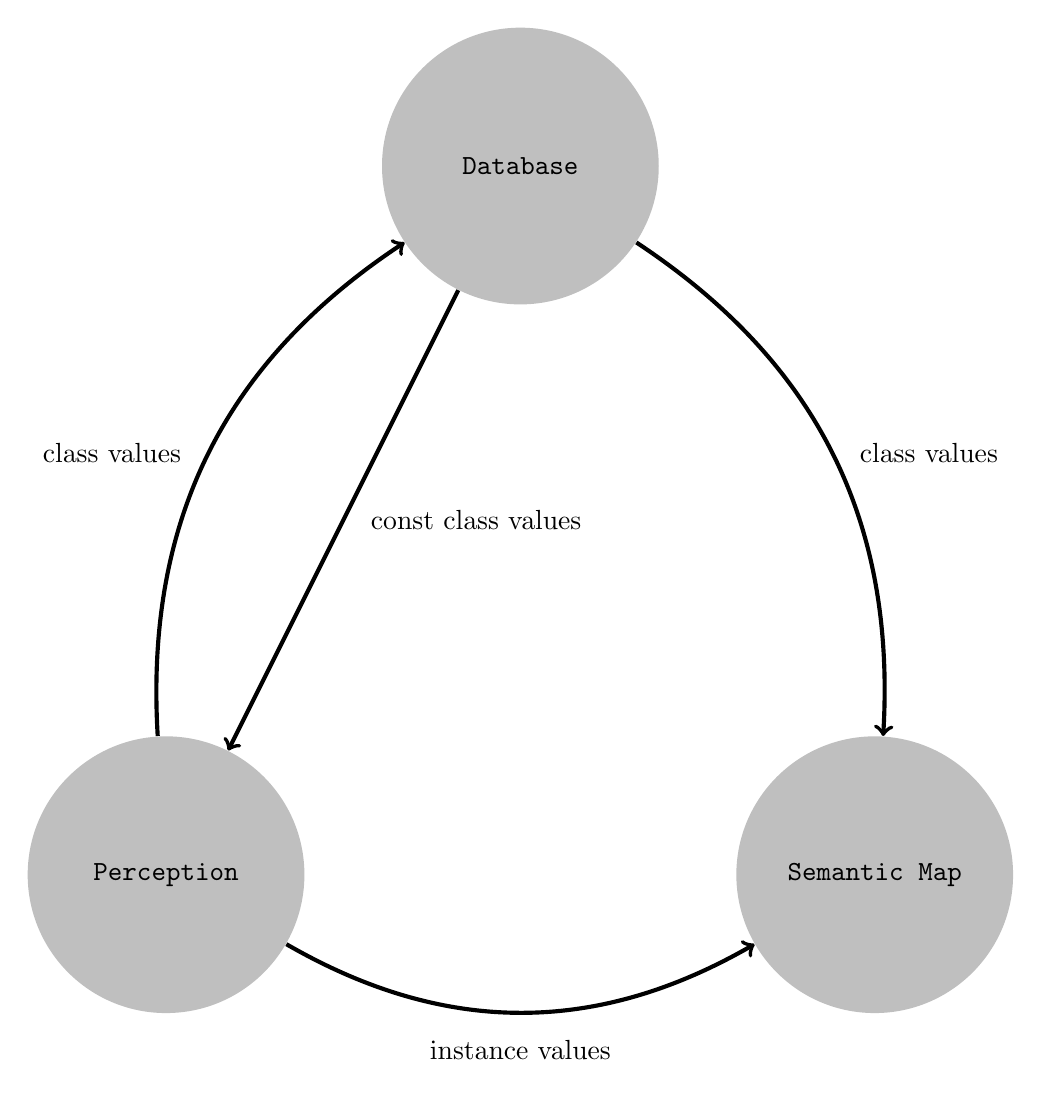
\begin{tikzpicture}[->, scale=1.8, auto, swap]
    % Draw the vertices.
    \node [vertex] (a) at (2.5, 5) {\texttt{Database}};
    \node [vertex] (b) at (  0, 0) {\texttt{Perception}};
    \node [vertex] (c) at (  5, 0) {\texttt{Semantic Map}};
    % Database <-> Perception.
    \path [edge] (a) edge [] node [right] {const class values} (b);
    \path [edge] (b) edge [bend left] node [left] {class values} (a);
    % Perception -> Semantic Map.
    \path [edge] (b) edge [bend right] node {instance values} (c);
    % Database -> Semantic Map.
    \path [edge] (a) edge [bend left] node [right] {class values} (c);
  \end{tikzpicture}
\end{figure}

\newpage
\subsection{Datatypes}
\subsection{Database}
\subsection{Perception}
\subsection{Semantic Map}
\subsection{Visualization}

\newpage
\section{Implementation}
\subsection{ROS}
\subsection{OpenCV}
\subsection{SiftGPU}
\subsection{PR2}
\subsection{RGB-D SLAM}
\subsection{Shared Library}
\subsection{Setup Samples}
\subsection{Mipmapping}
\subsection{Feature Detection and Matching}
\subsection{Filter Matches}
\subsection{Filter False Positives}
\subsection{Calculate 3D Pose}
\subsection{Memorise only new Objects}
\subsection{Evaluation Function}
\subsection{Tests}


\chapter{Analysis}
\section{Experimentation}
\section{Results}
\section{Evaluation}


\chapter{Discussion}


\chapter{Conclusion}


\chapter{Future Work / Outlook}


\end{document}
